\documentclass{article}

\usepackage{geometry}
\geometry{margin=1in}

\usepackage{graphicx}
\graphicspath{}

\title{STAT 778 Homework \#1: Kaplan-Meier Estimator in C\vspace{-2ex}}
\author{Tom Wallace}

\begin{document}

%\maketitle

\begin{center}
\LARGE STAT 778 HW 1: Kaplan-Meier Estimator in C

\large Tom Wallace

\large Spring 2018
\end{center}

\section{Program Structure}
There are three files. \texttt{misc.c} and its associated header file contain
miscellaneous utility functions (e.g. to create a vector). \texttt{km.c} contains
the \texttt{main} function and is where the more substantive code occurs.

\section{Compiling the Program}
The program must be compiled
with the \texttt{-lm} flag. An example of compilation on a Linux system:

\begin{center}
\texttt{gcc km.c misc.c -lm -o km}
\end{center}

\section{Using the Program}
The program is designed to read in data and output Kaplan-Meier survival
estimates and 95\% confidence intervals. The user must provide input and output
file arguments on the command line. Example:

\begin{center}
\texttt{km -i input\_file -o output\_file}
\end{center}

\section{Verification and Validation}
This program's computed Kaplan-Meier estimates and 95\% confidence intervals 
were compared to results obtained using the \texttt{survival} package in R. 
My C program produces nearly identical results.

\begin{center}
\begin{figure}[h!]
	\caption{Comparison of output}
	\centering
	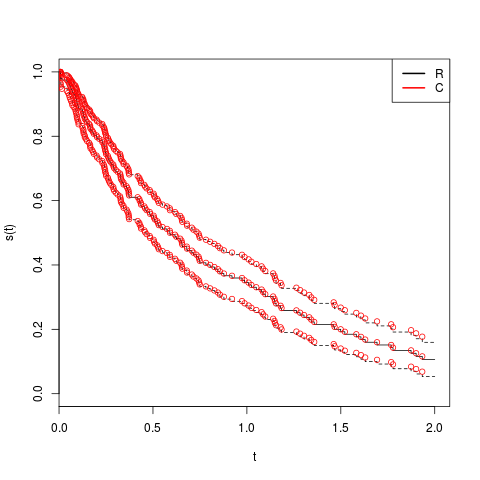
\includegraphics[scale=0.50]{comparison}
\end{figure}
\end{center}
\end{document}
